\section{结果}
\label{sec:results-zh}

\subsection{完整实验完成情况}

正式语料包含 20,000 个训练片段、2,000 个验证片段和 2,000 个测试片段，且 \texttt{smoke=false}。训练与评估环境为 Python 3.11.9、PyTorch 2.5.1+cu121 和可用的 CUDA，GPU 为 NVIDIA GeForce RTX 4060 Ti 16GB。13 个配置均在同一 2,000 条件测试集上评估，包括一个规则参照和 12 行神经结果；其中拟议的 $K=4$ 行与普通的 $K=1$ 行共享同一检查点。规范指标保存在 \path{results/project2_metrics.csv} 与 \path{results/project2_constraints.csv}，逐样例记录保存在 \path{results/project2_generation_examples.json}。

\subsection{共享生成器上的引导式候选选择}

将候选预算从 1 增至 4 并实施符号评分后，相对于对齐的首个候选，图示各选择指标均朝优选方向变化（表~\ref{tab:project2-main-results-zh}；图~\ref{fig:full-results-zh}a）。音级集合覆盖率由 0.9963 升至 0.9999，精确率由 0.9937 升至 1.0000；音程向量距离由 0.2390 降至 0.0045；循环序列顺序准确率由 0.1581 升至 0.2411，聚合完成率由 0.9949 升至 0.9969；节奏轮廓距离由 0.5113 降至 0.5041，姿态一致性由 0.4772 升至 0.4937。候选评分不可见的隐藏密度曲线误差也从 12.3501 描述性地降至 12.2353。

由于两行使用同一检查点，教师强制标记准确率均为 0.6686。两个解码器的严格序列变换准确率都保持为 0.0000。因此，候选选择改善了局部循环顺序遵循，但没有生成任何完整且精确的十二音形式。平均内容跨度比由 0.5024 升至 0.5195；尽管导出器补齐请求小节数，生成内容平均仍未覆盖近一半的请求时间跨度。

\begin{sidewaystable}[p]
\centering
\small
\resizebox{\textheight}{!}{%
\begin{tabular}{lrrrrrrrrrrrrrrr}
\toprule
实验 & 标记准确率 & PC覆盖率 & PC精确率 & IV距离 & 序列顺序 & 聚合完成 & 严格形式 & 节奏距离 & 密度误差 & 姿态一致 & 音域违反 & 内容跨度 & 有声声部 & XML解析 & XML小节 \\
\midrule
共享生成器，$K=4$ 引导 & 0.6686 & 0.9999 & 1.0000 & 0.0045 & 0.2411 & 0.9969 & 0.0000 & 0.5041 & 12.2353 & 0.4937 & 0.0000 & 0.5195 & 1.0000 & 1.0000 & 1.0000 \\
共享生成器，$K=1$ & 0.6686 & 0.9963 & 0.9937 & 0.2390 & 0.1581 & 0.9949 & 0.0000 & 0.5113 & 12.3501 & 0.4772 & 0.0000 & 0.5024 & 1.0000 & 1.0000 & 1.0000 \\
规则参照 & -- & 0.9988 & 1.0000 & 0.0260 & 1.0000 & 0.9958 & 0.9819 & 0.3021 & 2.9263 & 0.5683 & 0.0000 & 0.9986 & 1.0000 & 1.0000 & 1.0000 \\
\bottomrule
\end{tabular}
}
\caption{固定 2,000 条件程序化测试集上的自动结果。引导式和单候选行共享同一检查点，规则参照直接实现约束。序列顺序与严格形式准确率仅在序列条件样本上汇总。XML 解析和小节遵循率基于每个配置 20 次尝试导出；三行的 XML 声部数遵循率均为 1.0000。}
\label{tab:project2-main-results-zh}
\end{sidewaystable}


\begin{figure}[t]
  \centering
  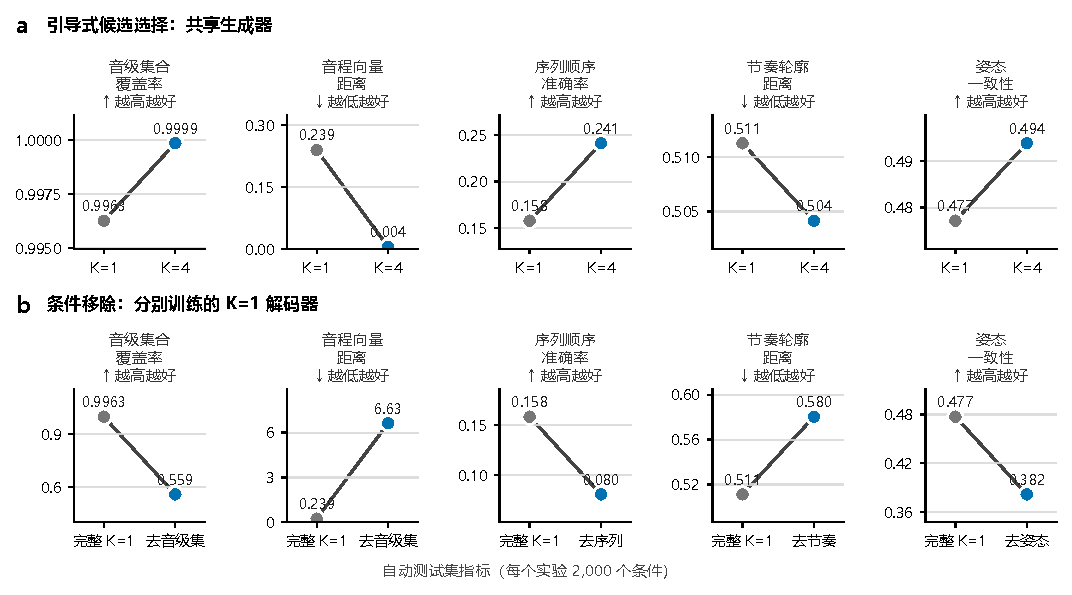
\includegraphics[width=\textwidth]{figures/project2_full_results_zh.pdf}
  \caption{固定 2,000 条件测试集上的自动约束效应。a：$K=1$ 与 $K=4$ 使用同一生成器和对齐的随机数流；$K=4$ 采样四个候选并实施符号评分。b：完整前缀模型与条件移除模型分别训练，均采用 $K=1$ 解码，并针对未改变的目标评估。箭头表示指标优选方向。所有结果均为单种子描述性自动指标，不是感知评分或推断统计。}
  \label{fig:full-results-zh}
\end{figure}

\subsection{条件字段与程序化参照}

相对于完整前缀的 $K=1$ 模型，从分别训练的 $K=1$ 模型中移除条件字段会使对应指标退化（图~\ref{fig:full-results-zh}b）。移除音级集合字段后，覆盖率由 0.9963 降至 0.5593，音程向量距离由 0.2390 升至 6.6267；移除序列字段后，序列顺序准确率由 0.1581 降至 0.0804；移除节奏字段后，节奏轮廓距离由 0.5113 升至 0.5803，隐藏密度误差由 12.3501 升至 13.6056；移除姿态字段后，姿态一致性由 0.4772 降至 0.3818。这些对比说明生成器在程序化分布内利用了对应的前缀字段，但不能据此推断模型可迁移到人类创作的独立作品。

规则参照直接实现指定程序，因此是构造参照，而不是学习基线。其序列顺序准确率为 1.0000，严格序列形式准确率为 0.9819；拟议神经解码器的对应值为 0.2411 和 0.0000。规则参照的节奏轮廓距离为 0.3021，密度误差为 2.9263，也低于神经解码器。这些差距表明，精确序列顺序和节奏实现仍是神经生成中的未解决问题。

\begin{sidewaystable}[p]
\centering
\small
\resizebox{\textheight}{!}{%
\begin{tabular}{lrrrrrrrrrrrrrrr}
\toprule
实验 & 标记准确率 & PC覆盖率 & PC精确率 & IV距离 & 序列顺序 & 聚合完成 & 严格形式 & 节奏距离 & 密度误差 & 姿态一致 & 音域违反 & 内容跨度 & 有声声部 & XML解析 & XML小节 \\
\midrule
无约束（种子 42） & 0.6668 & 0.7097 & 0.4970 & 24.4978 & 0.0838 & 0.5942 & 0.0000 & 0.5885 & 13.9216 & 0.4014 & 0.0000 & 0.4664 & 1.0000 & 1.0000 & 1.0000 \\
移除音级集合标记 & 0.6691 & 0.5593 & 0.5615 & 6.6267 & 0.1436 & 0.9951 & 0.0000 & 0.5119 & 12.3192 & 0.4754 & 0.0000 & 0.5043 & 0.9999 & 1.0000 & 1.0000 \\
移除序列标记 & 0.6688 & 0.9963 & 0.9928 & 0.2704 & 0.0804 & 0.9972 & 0.0000 & 0.5114 & 12.3576 & 0.4774 & 0.0000 & 0.5009 & 1.0000 & 1.0000 & 1.0000 \\
移除节奏标记 & 0.6673 & 0.9971 & 0.9932 & 0.2202 & 0.1513 & 0.9981 & 0.0000 & 0.5803 & 13.6056 & 0.4785 & 0.0000 & 0.4745 & 1.0000 & 1.0000 & 1.0000 \\
移除姿态标记 & 0.6686 & 0.9945 & 0.9961 & 0.2175 & 0.1559 & 0.9946 & 0.0000 & 0.5127 & 12.9772 & 0.3818 & 0.0000 & 0.4991 & 1.0000 & 1.0000 & 1.0000 \\
仅序列 & 0.6663 & 0.5696 & 0.5642 & 6.6106 & 0.0874 & 0.9973 & 0.0000 & 0.5852 & 13.9426 & 0.3879 & 0.0000 & 0.4612 & 1.0000 & 1.0000 & 1.0000 \\
仅音级集合 & 0.6662 & 0.9959 & 0.9936 & 0.2435 & 0.0817 & 0.9974 & 0.0000 & 0.5936 & 14.0748 & 0.3984 & 0.0000 & 0.4515 & 1.0000 & 1.0000 & 1.0000 \\
仅节奏 & 0.6679 & 0.7513 & 0.4836 & 28.2265 & 0.0812 & 0.6697 & 0.0000 & 0.5088 & 12.9737 & 0.3831 & 0.0000 & 0.4863 & 1.0000 & 1.0000 & 1.0000 \\
仅姿态 & 0.6677 & 0.7486 & 0.4833 & 28.2632 & 0.0838 & 0.6484 & 0.0000 & 0.5802 & 13.5792 & 0.4769 & 0.0000 & 0.4764 & 0.9999 & 1.0000 & 1.0000 \\
无约束（种子 53） & 0.6676 & 0.7264 & 0.4932 & 25.5506 & 0.0870 & 0.6019 & 0.0000 & 0.5767 & 13.7871 & 0.3850 & 0.0000 & 0.5109 & 1.0000 & 1.0000 & 1.0000 \\
\bottomrule
\end{tabular}
}
\caption{固定程序化测试集上的单候选条件前缀消融与聚焦条件模型。每个模型只接收其配置指定的前缀，但评估仍使用原始隐藏目标。序列顺序与严格形式准确率仅在序列条件样本上汇总。XML 解析和小节遵循率基于每个配置 20 次尝试导出；所有行的 XML 声部数遵循率均为 1.0000。}
\label{tab:project2-ablation-results-zh}
\end{sidewaystable}


\subsection{MusicXML 与可检查样例}

13 个配置共尝试导出 260 份 MusicXML，全部可解析并匹配请求的小节数和声部数。所有汇总行的音域违反率均为 0.0000；除两个聚焦消融中可忽略的舍入差异外，请求声部遵循率为 1.0000。拟议模型专家包在 \path{expert_eval/project2/} 下包含 20 份 MusicXML、20 份配对 JSON 报告、一份清单和空白盲评表。

图~\ref{fig:score-example-zh} 展示专家包中的一个拟议模型样例。其条件为音级集合 $\{0,1,2,5,6\}$、延续型节奏轮廓、音区扩张、四个声部和四个小节。自动报告记录音级集合覆盖率和精确率均为 1.0000，音程向量距离为 0.0000，节奏轮廓距离为 0.3125，姿态一致性为 0.7565，内容跨度比为 1.0000，且无音域违反。该样例只用于记谱层面的检查，不构成艺术质量证据。

\begin{figure}[t]
  \centering
  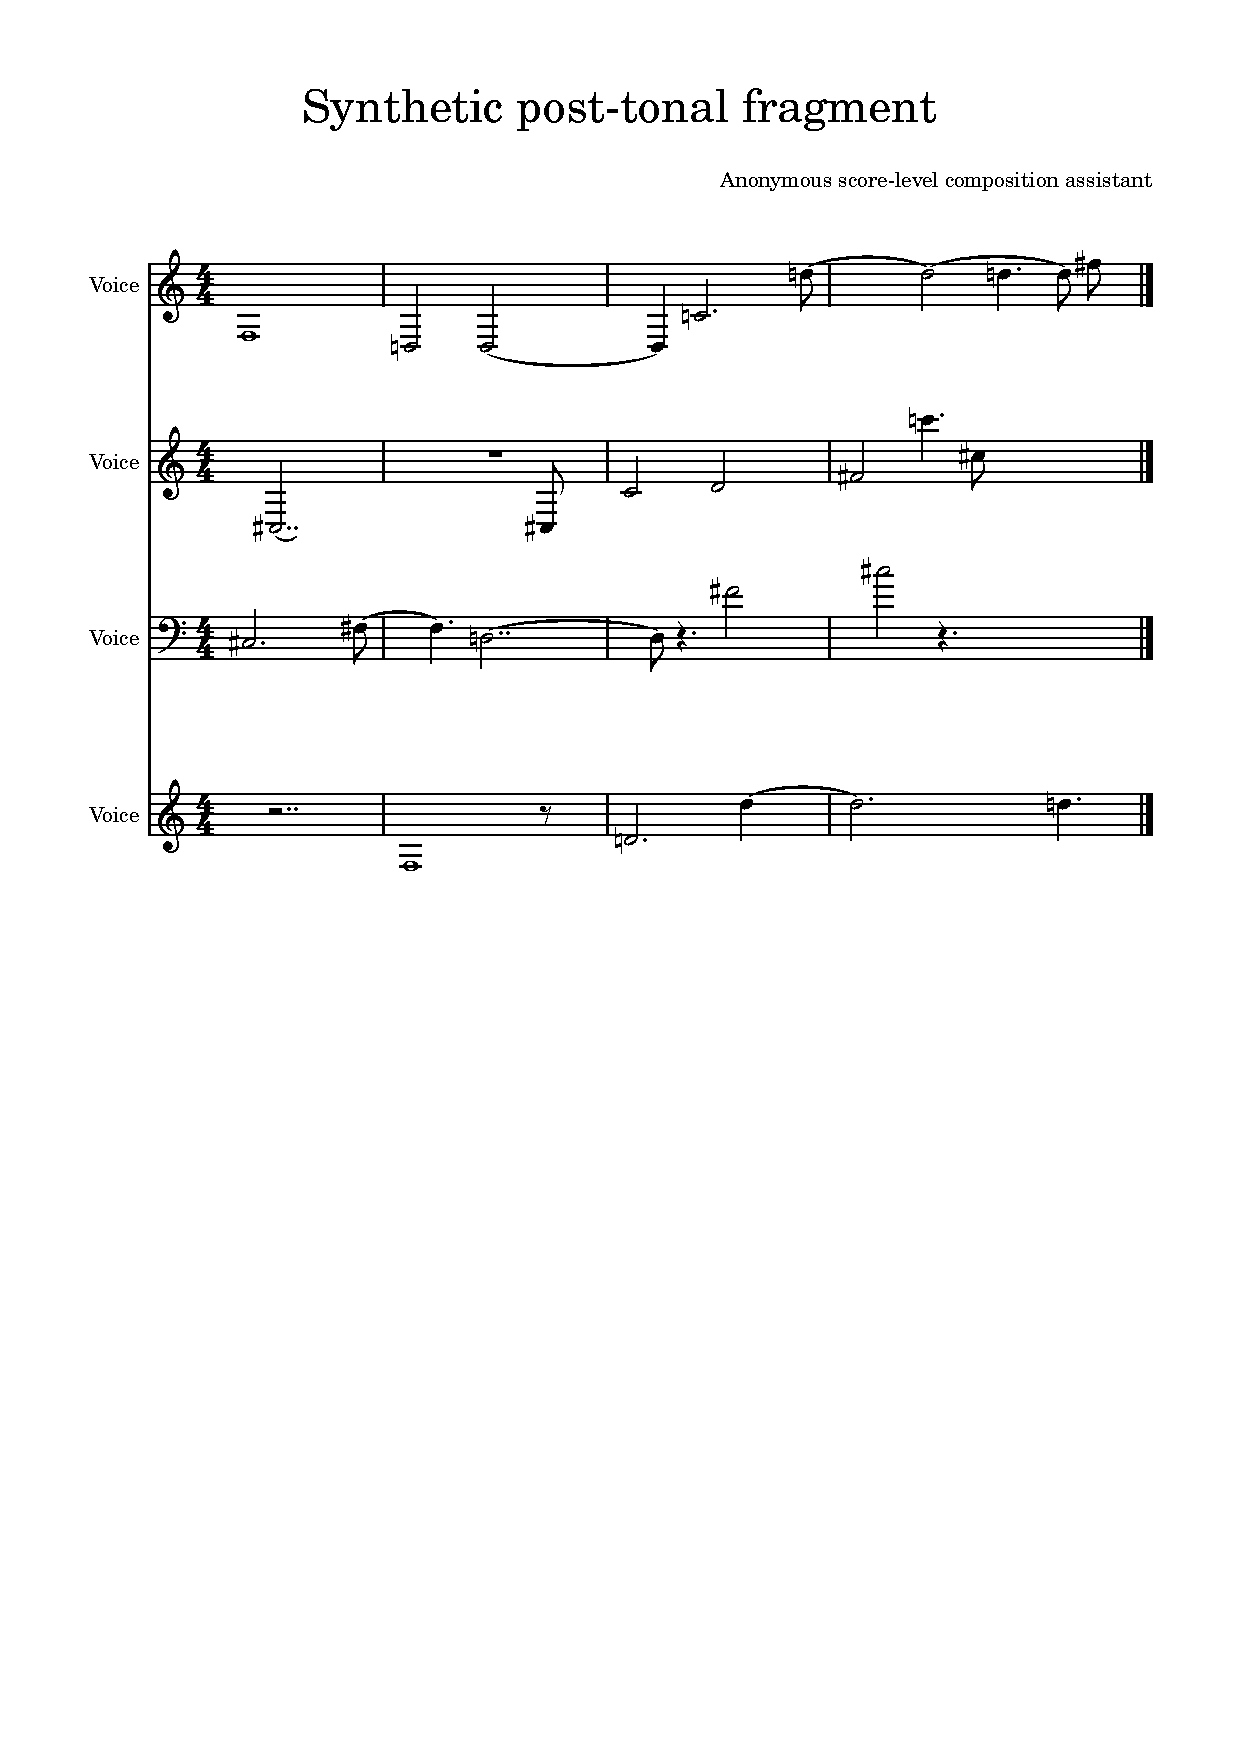
\includegraphics[width=0.96\textwidth,trim=35 360 35 35,clip]{figures/project2_full_score_example.pdf}
  \caption{拟议模型输出 \texttt{project2\_20}，由导出的 MusicXML 渲染。图中可见请求的四个声部和四个小节。留白、音区和时值均为模型生成的符号决策；该样例尚未获得任何人工偏好评分。}
  \label{fig:score-example-zh}
\end{figure}

\FloatBarrier
